\section{El lenguaje R}\label{introducciuxf3n-a-r}

\subsection{Introducción}

R \autocite{rlang} es un lenguaje de programación dirigido al tratamiento de datos, y
como tal proporciona estructuras de datos y funcionalidades básicas para
representar y tratar problemas de minería de datos. Es un proyecto GNU\footnote{GNU es un proyecto extenso que abarca distintos paquetes de software libre, R es uno de ellos: \url{https://www.gnu.org/}.}, y se considera una implementación alternativa del lenguaje S para estadística, desarrollado originalmente en Bell Labs.

Además, existe toda
una plataforma de paquetes para R denominada CRAN\footnote{\url{https://cran.r-project.org}}, que cuenta con
multitud de bibliotecas que facilitan tareas muy diversas, desde lectura y
visualización de datos hasta el propio procesamiento mediante distintos
algoritmos.

\subsection{Instalación}

Para utilizar el software desarrollado, será necesario instalar R junto con las utilidades de desarrollador del lenguaje. En general, hay disponibles paquetes binarios en los repositorios de las distribuciones más comunes de Linux, así como para Windows y macOS. Por ejemplo, para instalar R en distribuciones basadas en Debian como Ubuntu, ejecutaremos el siguiente comando:

\begin{verbatim}
sudo apt install r-base r-base-dev
\end{verbatim}

Los instaladores para Windows y macOS se pueden descargar desde el sitio web del proyecto R\footnote{\url{https://www.r-project.org/}}.

\subsection{Uso del lenguaje}

El lenguaje R se puede utilizar de forma interactiva mediante el REPL\footnote{Un REPL (\emph{read-eval-print-loop}) es un entorno de programación interactivo donde se evalúa el código línea a línea.} que se invoca con el comando \texttt{R}, mediante scripts que se pueden ejecutar con el programa \texttt{Rscript} o desde un IDE como RStudio \autocite{rstudio}.

R soporta la mayoría de tipos de dato básicos de cualquier otro lenguaje:
\begin{itemize}
\item \textit{logical}: valores lógicos entre \texttt{TRUE}, \texttt{FALSE} o \texttt{NA}
\item \textit{integer}: valores enteros
\item \textit{double}: valores reales de doble precisión (junto con \texttt{integer} forman el tipo \texttt{numeric})
\item \textit{complex}: números complejos
\item \textit{character}: cadenas de caracteres
\item \textit{raw}: datos binarios en bruto
\end{itemize}

Se caracteriza por el uso de algunas estructuras de datos: los vectores atómicos, las matrices, las listas y los \textit{data.frames}. Estos últimos son muy útiles para representar conjuntos de datos.

Las funciones son objetos de primera clase en R. Esto quiere decir que se pueden y suelen pasar como argumento a otras funciones, y devolver como valor de retorno. Esto permite el uso de funciones de orden superior clásicas del tipo \textit{map} o \textit{reduce}, que realizan operaciones simultáneamente sobre varios elementos de una estructura de datos.

R incorpora tres sistemas de orientación a objetos distintos: S3, S4 y \textit{Reference Classes} (RC). El primero de ellos es el más sencillo y el más utilizado, y es también el que se usa en el software desarrollado. Consiste simplemente en objetos tipo lista a los que se le ha aplicado un atributo de clase mediante la función \texttt{class}. Este atributo permite escoger un método cuando se realiza una llamada a una función genérica.

\begin{example}
  Para realizar una demostración sobre la orientación a objetos S3 de R, vamos a definir objetos de clase \texttt{animal} que implementen el método \texttt{print}. Este es ya una función genérica de R, luego la asociación del método que definamos con nuestros objetos será automática. Para crearlos, podemos usar una función que hará las veces de constructor:
  \begin{lstlisting}
animal <- function(nombre, sonido) {
  objeto <- list(
    nombre = nombre,
    sonido = sonido
  )
  class(objeto) <- "animal"
  return(objeto)
}
print.animal <- function(animal) {
  print(paste("Soy un", animal$nombre, "y hago", animal$sonido))
}
print(animal("gato", "miau"))
# => [1] "Soy un gato y hago miau"
print(animal("perro", "guau"))
# => [1] "Soy un perro y hago guau"
\end{lstlisting}

Nótese que en las líneas 12 y 14 del código anterior se llama a la función \texttt{print}, que al ser genérica busca el método correspondiente para los objetos de clase \texttt{animal}.
\end{example}

\section{La biblioteca MXNet}\label{sec:mxnet}
\subsection{Descripción}
MXNet \autocite{mxnet} es una biblioteca de algoritmos de Deep Learning, es decir, incluye la funcionalidad necesaria para construir estructuras de aprendizaje profundas, calcular los gradientes con propagación hacia atrás (sección \ref{sec:backprop}), entrenarlas con datos de entrada mediante los algoritmos de optimización estudiados en la sección \ref{sec:dl-opt} y realizar predicciones sobre nuevos datos.

Frente a otras bibliotecas similares como Tensorflow \autocite{tensorflow} o Theano \autocite{theano}, el motor de MXNet está escrito en el lenguaje C++, lo que reduce los tiempos de ejecución. Sin embargo, esto no limita su uso puesto que proporciona acceso a las funcionalidades mediante APIs para otros lenguajes como Python, Scala o R.

Esta biblioteca permite ejecutar los algoritmos de forma secuencial, distribuida o en dispositivos GPU. Además, proporciona dos mecánicas de programación diferenciadas: simbólica e imperativa. Por un lado, la programación simbólica permite diseñar un modelo de forma rápida sin necesidad de aportar los datos de entrada \textit{a priori} ni ejecutar los algoritmos de forma inmediata. Esto permite una programación más flexible, pudiendo acceder a los parámetros y modificarlos de forma desconectada de los cálculos costosos. Por otro lado, la programación imperativa facilita el control sobre los procesos de aprendizaje y la forma en que los datos se propagan por una red neuronal.

\subsection{Instalación}

Para disponer de MXNet en un ordenador y poder usarla desde R, es necesario compilar e instalar tanto la biblioteca como el paquete compañero para R. Las dependencias son las herramientas de compilación básicas (G++, GNU Make) y una implementación de la biblioteca de álgebra lineal BLAS. como OpenBLAS o ATLAS. Opcionalmente se puede instalar OpenCV para facilitar el tratamiento de imágenes. Tras esto, se ejecutan los siguientes comandos para descargar y compilar el software:

\begin{lstlisting}[language=sh,frame=none]
git clone --recursive https://github.com/dmlc/mxnet
cd mxnet
cp make/config.mk . # editar las entradas necesarias
make -j $(nproc)
sudo install -D lib/libmxnet.so /usr/lib/libmxnet.so
\end{lstlisting}
%$ <-- hack for emacs syntax highlighting

Si se desea soporte para cómputo sobre GPU con CUDA, se añadirán las opciones \texttt{USE\_CUDA=1} \texttt{USE\_CUDA\_PATH=/opt/cuda} \texttt{USE\_CUDNN=1} al archivo \texttt{config.mk}, utilizando el camino conveniente para la biblioteca CUDA.

Alternativamente, en sistemas basados en Arch Linux basta con instalar el paquete \texttt{mxnet}\footnote{\url{https://aur.archlinux.org/packages/mxnet/}} del repositorio de usuarios AUR.

Por último, para instalar el paquete compañero para R, se utilizan las siguientes órdenes de línea de comandos desde el directorio donde se ha clonado el repositorio:

\begin{lstlisting}[language=sh,frame=none]
make rpkg
R CMD INSTALL mxnet_current_r.tar.gz
\end{lstlisting}

\subsection{Uso de la biblioteca}
Para construir una estructura de aprendizaje profunda con MXNet, basta con comenzar con un símbolo que corresponderá a los datos de entrada, después especificar las capas que formarán la red y, por último, el tipo de salida deseada.

Después, para ajustar el modelo creado con un conjunto de entrenamiento, MXNet proporciona algunas utilidades de alto nivel y otras más cercanas al cómputo paso a paso de las propagaciones hacia adelante y hacia atrás. De las primeras podemos destacar \texttt{mx.model.FeedForward.create} y de las últimas \texttt{mx.exec.backward} y \texttt{mx.exec.forward}.

\begin{example}

  En este ejemplo vamos a construir una red prealimentada sencilla que permitirá aproximar el cálculo de la hipotenusa de un triángulo rectángulo a partir de las longitudes de los catetos.

  Primero, comenzamos construyendo la red. Creamos la variable simbólica que contendrá los datos y la enlazamos con dos capas ocultas de 2 y 10 unidades respectivamente, y con la capa de salida que aproximará la hipotenusa, evaluará la pérdida y permitirá realizar el aprendizaje.
  
\begin{lstlisting}[language=R,frame=none]
library(mxnet)
red <- mx.symbol.Variable("data")
red <- mx.symbol.FullyConnected(red, num_hidden = 2)
red <- mx.symbol.Activation(red, act_type = "relu")
red <- mx.symbol.FullyConnected(red, num_hidden = 10)
red <- mx.symbol.Activation(red, act_type = "relu")
red <- mx.symbol.FullyConnected(red, num_hidden = 1)
red <- mx.symbol.LinearRegressionOutput(red)
\end{lstlisting}
  
  Ahora, creamos los datos de entrada: aleatoriamente escogemos catetos y después calculamos la hipotenusa en la variable \texttt{label}. Separamos en un conjunto para entrenamiento y otro para test. De forma similar, podríamos también proceder con una validación cruzada.
  
\begin{lstlisting}[language=R,frame=none]
set.seed(42)
mx.set.seed(42)

input <- data.frame(
  cat1 = round(runif(100, min = 1, max = 10)),
  cat2 = round(runif(100, min = 1, max = 10)))
x = t(data.matrix(input))
label <- sqrt(input$cat1 ** 2 + input$cat2 ** 2)
train_x <- x[,1:74]
train_y <- label[1:74]
test_x <- x[,75:100]
test_y <- label[75:100]
\end{lstlisting}

Por último, entrenamos el modelo que creamos anteriormente, escogiendo los parámetros del proceso de aprendizaje, en particular el optimizador SGD explicado en la sección \ref{sec:sgd}, y obtenemos las predicciones sobre el conjunto de test.
  
\begin{lstlisting}[language=R,frame=none]
model <- mx.model.FeedForward.create(
  symbol = red,
  X = train_x,
  y = train_y,
  num.round = 240,
  array.layout = "colmajor",
  optimizer = "sgd",
  learning.rate = 0.015,
  momentum = 0.2,
  eval.metric = mx.metric.rmse
)
# => Train-rmse=0.693727073714297
predict(model, test_x)
\end{lstlisting}
  
\end{example}


\section{Introducción a Ruta}\label{el-paquete-ruta}

Se ha desarrollado un paquete software, denominado Ruta, con el
objetivo de proporcionar acceso a diversas estructuras de aprendizaje profundo no supervisado de forma muy sencilla. El paquete se ha escrito en el lenguaje R utilizando los recursos de la biblioteca MXNet.

\subsection{Desarrollo y metodologías}\label{metodologuxeda-de-desarrollo}

Al comienzo del desarrollo del software, se han analizado los objetivos perseguidos y se han escogido las tecnologías que nos facilitarían su consecución. En concreto, se ha elegido el lenguaje R por varias razones. Por un lado apenas dispone de herramientas de Deep Learning cómodas y consolidadas, luego este nuevo software no es redundante con nada existente. Además, R es un lenguaje que aporta muchas facilidades para la visualización de datos, lo cual es beneficioso ya que parte del software desarrollado se dedica a eso. También se eligió la biblioteca MXNet tras comparar con varias de las competidoras en el mercado en ese momento: Tensorflow se descartó por ser relativamente más lenta que el resto, y Theano y Caffe no disponían de API para R, mientras que otras librerías no estaban tan desarrolladas y no aportaban la funcionalidad que necesitábamos.

La metodología de desarrollo ha sido de tipo ágil, es decir, se ha desarrollado partiendo de un prototipo funcional, alterando y aumentando sus funcionalidades según se ha ido requiriendo. La documentación\footnote{Se puede consultar desde R mediante \texttt{?} delante del nombre de la función. Por ejemplo, \texttt{?ruta.makeTask}.} es exhaustiva en el sentido de que cubre toda la funcionalidad disponible para el usuario, pero no es excesiva. Además, progresivamente se ha ido adaptando el desarrollo según las nuevas necesidades o los obstáculos encontrados.

Un prototipo preliminar de esta herramienta, con funcionalidades básicas de entrenamiento de autoencoders y visualizaciones sencillas, se implementó bajo el nombre \emph{dlvisR} y se presentó en el congreso nacional CAEPIA 2016 \autocite{charte2016dlvisr}.

Puesto que se trata de un software científico que se sostiene sobre varias piezas de software libre, se ha decidido que también esta herramienta será de código abierto y libre. Para asegurar que se mantiene libre, además, se ha utilizado la licencia \textit{GNU General Public License} (GPL) 3.0, que requiere que las modificaciones que se realicen sobre el código del software se liberen bajo la misma licencia\footnote{Texto de la licencia disponible en \url{https://www.gnu.org/licenses/gpl.html}.}. Así, el código del software está publicado en el repositorio fdavidcl/ruta de GitHub\footnote{\url{https://github.com/fdavidcl/ruta/}}.

Para asistir a la comprobación del software completo durante su desarrollo, se ha utilizado un sistema de integración continua, es decir, automatización de \textit{builds} y de tests. Este sistema realiza, a cada avance publicado en GitHub, una comprobación mediante el programa \texttt{R CMD check}.

\subsection{Instalación}

Para instalar la última versión estable de Ruta y el paquete compañero Rutavis, basta con utilizar el conocido paquete \texttt{devtools} \autocite{devtools} para realizar automáticamente la descarga y la instalación. Desde la consola de R ejecutamos:
\begin{lstlisting}[numbers=none]
devtools::install_github("fdavidcl/ruta")
devtools::install_github("fdavidcl/rutavis")
\end{lstlisting}

Una vez instalado, para cargarlos utilizamos las órdenes siguientes:
\begin{lstlisting}[numbers=none]
library(ruta)
library(rutavis)
\end{lstlisting}


\section{Componentes del paquete y uso}\label{componentes-del-paquete}

\subsection{Estructura}

El software se estructura como un paquete convencional de R, siguiendo la jerarquía de directorios siguiente:
\begin{itemize}
\item \texttt{man/}
  \begin{itemize}
  \item archivos de documentación en formato \texttt{.Rd}.
  \end{itemize}
\item \texttt{R/}
  \begin{itemize}
  \item \texttt{autoencoder\_learner.R}: implementa la generación de redes profundas tipo autoencoder.
  \item \texttt{autoencoder\_model.R}: incluye el entrenamiento de autoencoders y las herramientas de análisis de modelos.
  \item \texttt{classes.R}: incluye las clases utilizadas a lo largo del paquete.
  \item \texttt{learner.R}: incluye las funcionalidades comunes a los algoritmos de aprendizaje.
  \item \texttt{model.R}: implementa funcionalidades comunes a los modelos.
  \item \texttt{rbm\_learner.R}: implementa la generación de máquinas de Boltzmann restringidas.
  \item \texttt{rbm\_model.R}: incluye el entrenamiento de RBMs.
  \item \texttt{task.R}:  contiene las funcionalidades comunes a las tareas.
  \item \texttt{unsupervised\_task.R}: implementa la gestión de tareas no supervisadas. 
  \item \texttt{util.R}: incluye utilidades adicionales.
  \end{itemize}
\item \texttt{DESCRIPTION}: indica metadatos del paquete, como nombre, versión y dependencias.
\item \texttt{LICENSE}: contiene el texto de la licencia libre, en este caso GPL 3.0.
\item \texttt{NAMESPACE}: da información sobre los nombres de funciones exportadas e importadas.
\end{itemize}

\subsection{Funcionalidad}

Las funcionalidades del paquete se han dividido en tres categorías:
\begin{itemize}
\item Tareas
\item Algoritmos de aprendizaje
\item Modelos entrenados
\end{itemize}
Aquí se ha utilizado como guía la arquitectura del paquete \texttt{mlr} \autocite{mlr} dirigido a aprendizaje automático en general.

Por un lado, las tareas representan conjuntos de datos de los que se desea aprender un modelo. Para ello, se construirán representaciones de los algoritmos de aprendizaje, ajustadas con diversos parámetros, que después se podrán entrenar y generar un modelo. Dicho modelo se podrá estudiar para obtener información sobre nuevos datos o sobre los aprendidos.

\subsection{Tareas}

Una tarea de aprendizaje se compone de un conjunto de datos y varios metadatos que aportan información acerca del mismo. En Ruta se pueden crear tareas genéricas con la función \texttt{ruta.makeTask} y tareas de aprendizaje no supervisado con \texttt{ruta.makeUnsupervisedTask}.

\begin{example}
  Construyamos una tarea de aprendizaje no supervisado a partir del conocido conjunto de datos Iris \autocite{fisher1936iris}. Para ello, será necesario cargar el conjunto y posteriormente generaremos una tarea de Ruta, indicando la columna en la que se encuentra la clase, y podremos obtener información sobre ella:
  \begin{lstlisting}
data(iris)
task <- ruta.makeUnsupervisedTask("iris", data = iris, cl = 5)
print(task)
# ruta Task: iris
# Type: unsupervised
# Instances: 150
# Features: 5
# Has class: Yes (5)
  \end{lstlisting}
\end{example}

\subsection{Algoritmos de aprendizaje}

En el momento actual del desarrollo, Ruta cuenta con una implementación de autoencoders basada en la biblioteca MXNet y una implementación básica de RBMs. Para utilizarlas, se dispone de la función \texttt{ruta.makeLearner} que da acceso a las técnicas de aprendizaje implementadas. Además, para generar modelos a partir de algoritmos y tareas, basta con utilizar el método \texttt{train} que se ha especializado para los objetos de clase \texttt{``rutaAutoencoder''}.

\begin{example}\label{ex:ruta2}
  Utilizamos la función mencionada para crear un objeto que represente un autoencoder de 5 capas de 4, 10, 2, 10 y 4 unidades respectivamente, con activaciones ReLU.

  Lo entrenamos con la tarea que creamos anteriormente, seleccionando el optimizador Adam (\autoref{alg:adam}) con una tasa de aprendizaje de $0.005$:
  \begin{lstlisting}
ae <- ruta.makeLearner("autoencoder",
                       hidden = c(4, 10, 2, 10, 4),
                       activation = "relu")
print(ae)
# ruta Learner
# Type: Autoencoder
# Backend: mxnet
# Sparse: No

model <- train(ae, task,
               epochs = 500,
               learning.rate = 0.005,
               optimizer = "adam")
  \end{lstlisting}
\end{example}

Destacamos algunos parámetros interesantes en el ejemplo anterior. Primero, \texttt{activation}, que indica la función de activación que llevarán las unidades de la red. Las funciones de activación disponibles son:
\begin{itemize}
\item Ninguna (unidad lineal): \texttt{NULL}
\item ReLU: \texttt{``relu''}
\item Función logística: \texttt{``sigmoid''}
\item Función \emph{softplus}: \texttt{``softrelu''}
\item Función tangente hiperbólica: \texttt{``tanh''}
\item Tipo \emph{leaky} ReLU: \texttt{``leaky''}, \texttt{``elu''}, \texttt{``prelu''}, \texttt{``rrelu''}
\end{itemize}

Por otra parte, el parámetro \texttt{optimizer} permite escoger el algoritmo de optimización con el que se entrenará. Los optimizadores disponibles son:
\begin{itemize}
\item Gradiente descendiente estocástico (\autoref{alg:sgd}): \texttt{``sgd''}
\item Adagrad (\autoref{alg:adagrad}): \texttt{``adagrad''}
\item RMSProp (\autoref{alg:rmsprop}): \texttt{``rmsprop''}
\item Adam (\autoref{alg:adam}): \texttt{``adam''}
\end{itemize}
Cada uno de ellos acepta además los parámetros adicionales propios del algoritmo correspondiente.

\subsection{Modelos entrenados}

Una vez se ha obtenido  un modelo entrenado, se pueden realizar distintas operaciones sobre él. Una de las más interesantes es obtener las codificaciones para unos datos dados, es decir, las salidas de la capa interna del autoencoder. Para ello contamos con la función \texttt{ruta.deepFeatures}. Adicionalmente, la función \texttt{ruta.layerOutputs} permite extraer las salidas de cualquier capa de la red. Por último, la implementación del método \texttt{predict} para objetos de clase \texttt{``rutaModel''} facilita las salidas de la última capa del autoencoder.

\begin{example}
Ahora tomamos el modelo aprendido en el \autoref{ex:ruta2} y obtenemos, para los mismos datos con los que se entrenó, las codificaciones en la capa interna:
  \begin{lstlisting}
deepf <- ruta.deepFeatures(model, task)
# Extracting layer aelayer3act_output (output #13)
# Setting arguments up to aelayer3_bias (arg #6)
  \end{lstlisting}
\end{example}

Para conseguir extraer estas características internas, ha sido necesaria la implementación de una funcionalidad ausente en la API de MXNet para R: la predicción de capas internas de una red. Dicha implementación se encuentra también incluida en el paquete como la función \texttt{predictPartial}. Esta función trabaja a bajo nivel, controlando la propagación de datos a través de cada capa.

\section{Visualización con Rutavis}\label{sec:rutavis}

Una herramienta complementaria a \texttt{ruta} es \texttt{rutavis}, una
aplicación con interfaz de usuario web que permite componer
visualizaciones de forma interactiva y compararlas.

\subsection{Estructura}

De nuevo, este software se estructura como un paquete convencional de R, siguiendo una jerarquía similar a Ruta pero con algunas diferencias:
\begin{itemize}
\item \texttt{inst/}
  \begin{itemize}
  \item \texttt{shiny/}
  \begin{itemize}
  \item \texttt{www/}
  \begin{itemize}
  \item archivos adicionales para la interfaz web (CSS y JavaScript).
  \end{itemize}
  \item \texttt{template.html}: plantilla HTML que compone la web.
  \item \texttt{server.R}: script que ejecuta el servidor web.
  \item \texttt{ui.R}: script que compone la interfaz del cliente mediante la plantilla.
  \end{itemize}
  \end{itemize}
\item \texttt{man/}
  \begin{itemize}
  \item archivos de documentación en formato \texttt{.Rd}.
  \end{itemize}
\item \texttt{R/}
  \begin{itemize}
  \item \texttt{gui.R}: implementa el lanzamiento del servidor web.
  \item \texttt{plots.R}: implementa distintos tipos de gráficos para representar modelos.
  \end{itemize}
\item \texttt{DESCRIPTION}: indica metadatos del paquete, como nombre, versión y dependencias.
\item \texttt{LICENSE}: contiene el texto de la licencia libre, en este caso GPL 3.0.
\item \texttt{NAMESPACE}: da información sobre los nombres de funciones exportadas e importadas.
\end{itemize}

\subsection{Funcionalidad}

Rutavis es un paquete totalmente dependiente de Ruta, centrado exclusivamente en la generación de gráficos a partir de modelos entrenados. Cumple dos responsabilidades principales: por una parte, la gestión de visualizaciones que ayuden a entender el comportamiento de las técnicas no supervisadas y de los modelos que entrenan; por otra, una interfaz web que facilita al usuario la creación de dichas visualizaciones.

Los gráficos generados se muestran mediante la herramienta de visualización Plotly \autocite{plotly}, que tiene una amplia gama de gráficas y una extensa documentación. Cuenta también con un paquete homónimo para R.

Además, para la creación del servidor web y la aplicación web desde R, se ha aprovechado el paquete Shiny \autocite{shiny}, que proporciona diversas utilidades para el intercambio de datos entre el cliente y el servidor. Se ha utilizado el \emph{framework} CSS Bulma\footnote{\url{http://bulma.io}} para dar estructura y estilo a los elementos de la página. La interactividad con el usuario se ha programado en JavaScript en el cliente, que envía los datos al servidor y gestiona las respuestas.

\subsection{Uso de la aplicación}\label{uso-de-la-aplicaciuxf3n}

Con Rutavis se pueden crear gráficos sin necesidad de hacer uso de la interfaz web, mediante la implementación de la función genérica \texttt{plot} para objetos de clase \texttt{``rutaModel''}.

\begin{example}
  Con una tarea y un modelo como los utilizados anteriormente para el conjunto de datos iris, vamos a generar un gráfico que muestre las salidas codificadas mediante la capa intermedia del autoencoder. Utilizamos el método \texttt{plot.rutaModel} y le pasamos las mismas instancias con las que se entrenó:
\begin{lstlisting}[numbers=none]
plot(model, task)
\end{lstlisting}
\begin{figure}[hbtp]
  \centering
  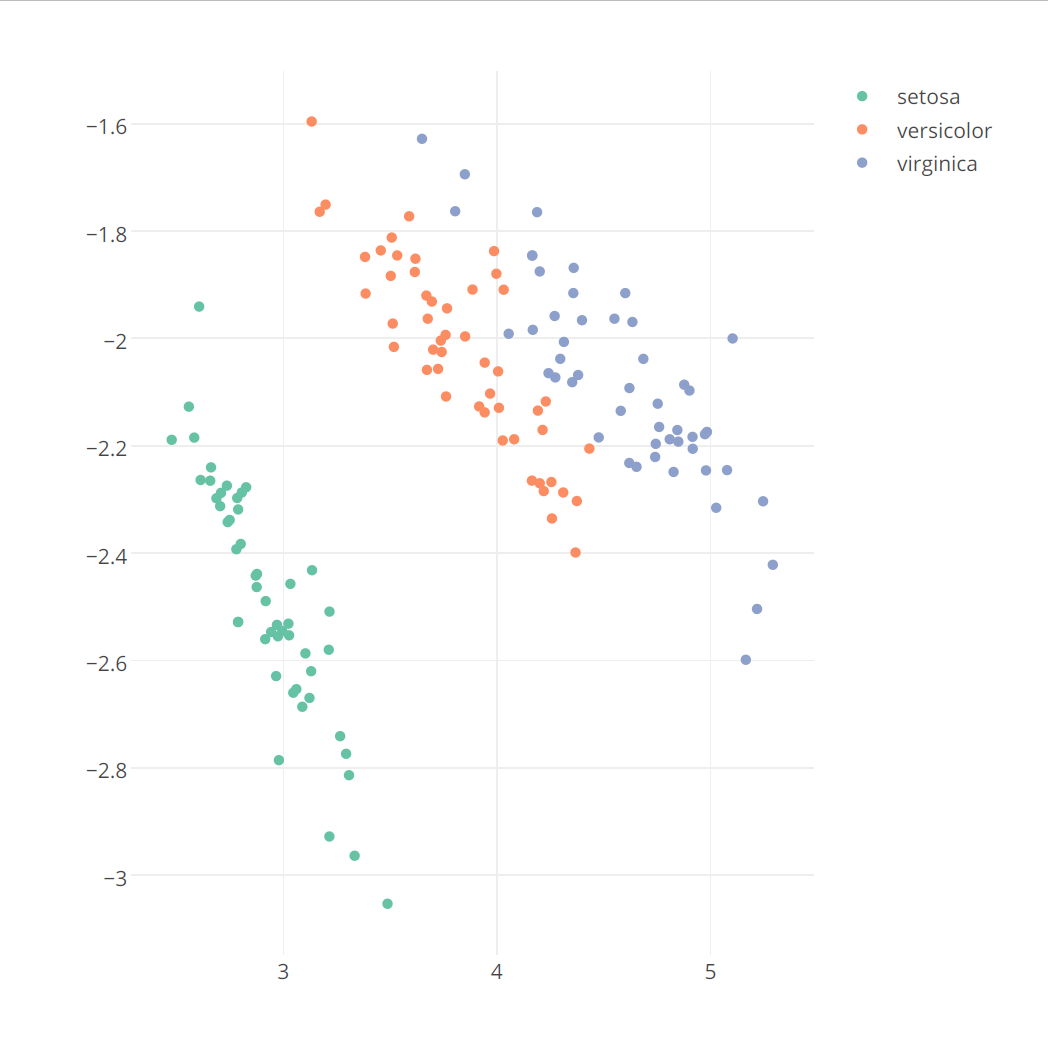
\includegraphics[width=0.8\textwidth]{images/rutavis_iris.png}
  \caption{\label{fig:irisplot}Gráfico de la codificación de los datos de entrada mediante la capa interna del autoencoder}
\end{figure}

La salida será un gráfico del estilo del de la \autoref{fig:irisplot}. 
Como se puede observar, el autoencoder consigue comprimir gran parte de la información de las 4 variables de Iris en solamente 2. Pese a no haber utilizado información sobre la clase, la representación bidimensional del conjunto de datos mantiene el bajo solapamiento entre clases.
\end{example}

Para lanzar la interfaz de usuario web, simplemente hay que ejecutar la siguiente llamada:
\begin{lstlisting}[numbers=none]
rutavis::ruta.gui()
\end{lstlisting}

Se abrirá una pestaña de navegador con la interfaz de usuario, inicialmente en la pantalla mostrada en la \autoref{fig:rutavis-welcome}, que nos permitirá crear una nueva visualización. Se pueden gestionar simultáneamente varias visualizaciones, de forma que se puedan estudiarse una a una y modificar sus parámetros, ver comparativamente en formato mosaico, o listar en estilo \emph{notebook} junto a los parámetros establecidos.

\begin{figure}[hbtp]
  \centering
  \fbox{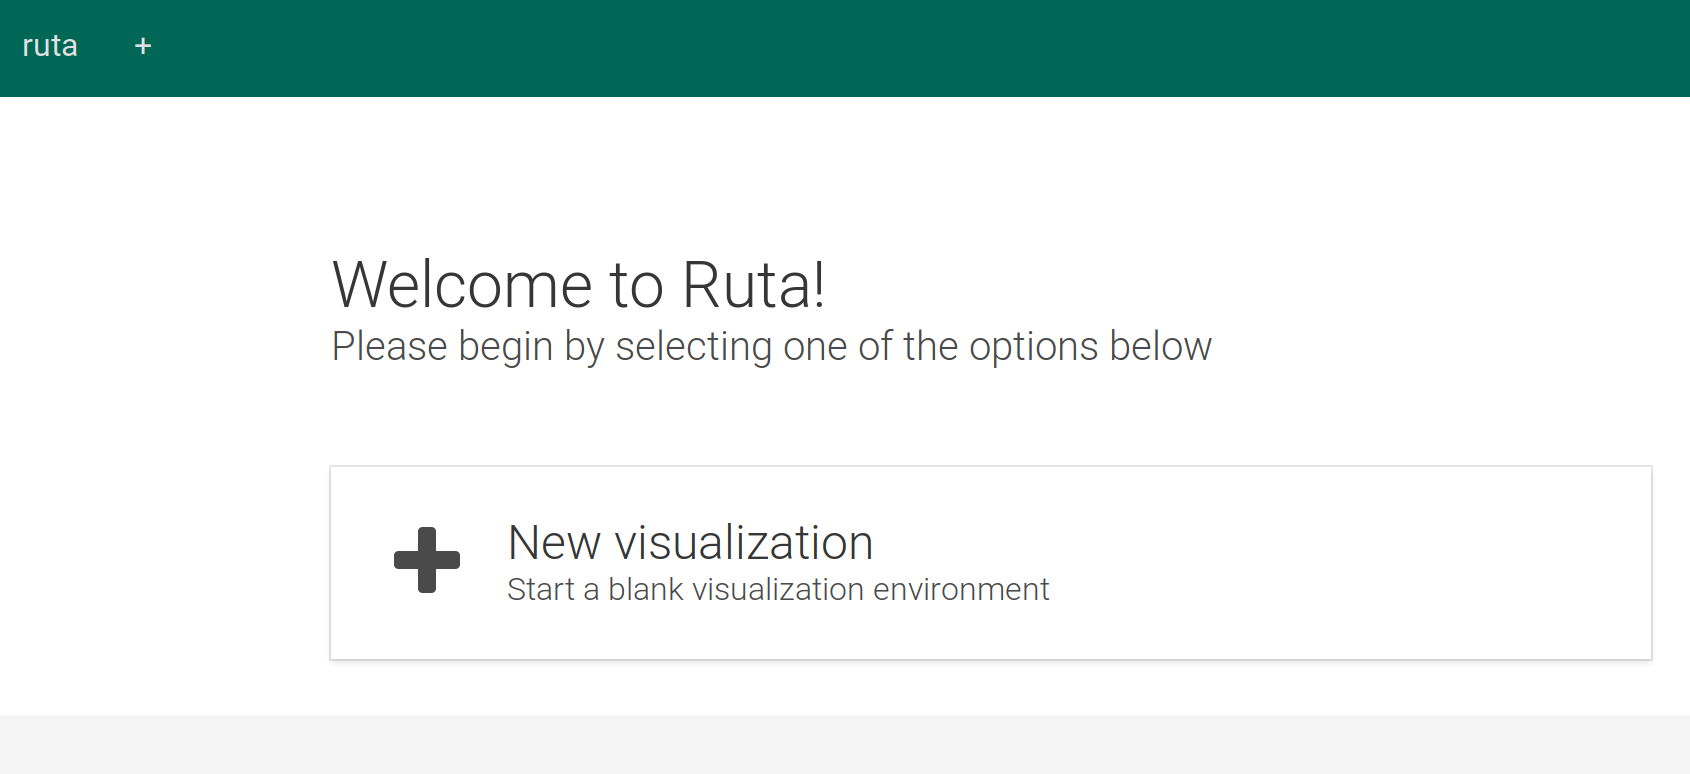
\includegraphics[width=0.8\textwidth]{images/rutavis_welcome}}
  \caption[Interfaz gráfica de Rutavis]{Pantalla de bienvenida de Rutavis}
  \label{fig:rutavis-welcome}
\end{figure}

Vamos a realizar paso a paso un entrenamiento de dos modelos basados en autoencoders para el conjunto de datos WDBC (\emph{Wisconsin Diagnostic Breast Cancer}) obtenido de \autocite{Lichman:2013}. El conjunto representa un problema de clasificación binaria, donde a partir de características médicas se pretende predecir si un tumor es benigno o maligno.

Comenzamos lanzando la interfaz web y seleccionando la opción \emph{New visualization}. Se abrirá una vista compuesta por un panel de ajustes y un espacio para los gráficos. Cargamos el conjunto de datos mediante la opción \emph{Upload new dataset} del panel. Seleccionamos la característica que corresponde con la clase de la lista \emph{Class attribute}.

Para configurar un modelo de aprendizaje, escogemos los parámetros deseados. Como se puede observar en el ejemplo de la \autoref{fig:rutavis2}, utilizamos capas con unidades de tipo \emph{leaky} ReLU, una codificación en 3 variables, un entrenamiento con AdaGrad de 200 épocas ajustando la tasa de aprendizaje a $0.02$. En la \autoref{fig:rutavis1} se muestra la vista de visualización única con el gráfico resultante, que corresponde a la salida de la capa interna del autoencoder respecto a los datos de entrada (los puntos verdes corresponden a tumores benignos y los azules a malignos). Se trata de un gráfico interactivo, sobre el que podemos arrastrar el ratón para mover los ejes, acercar o alejar la vista, y guardar en formato PNG.

\begin{figure}[hbtp]
  \centering
  \fbox{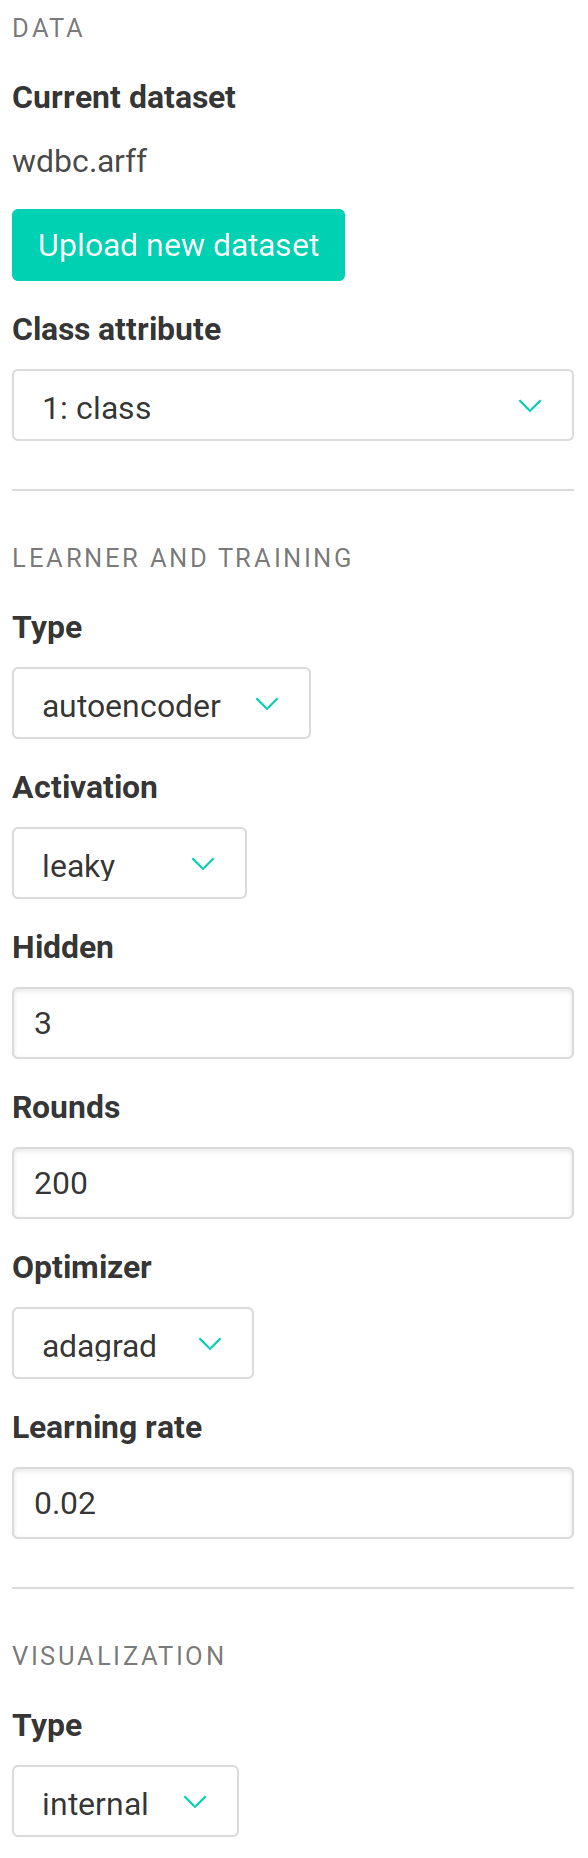
\includegraphics[width=0.4\textwidth]{images/rutavis_params}}
  \caption[Interfaz gráfica de Rutavis]{El panel de ajuste de parámetros en detalle}
  \label{fig:rutavis2}
\end{figure}

\begin{figure}[hbtp]
  \centering
  \fbox{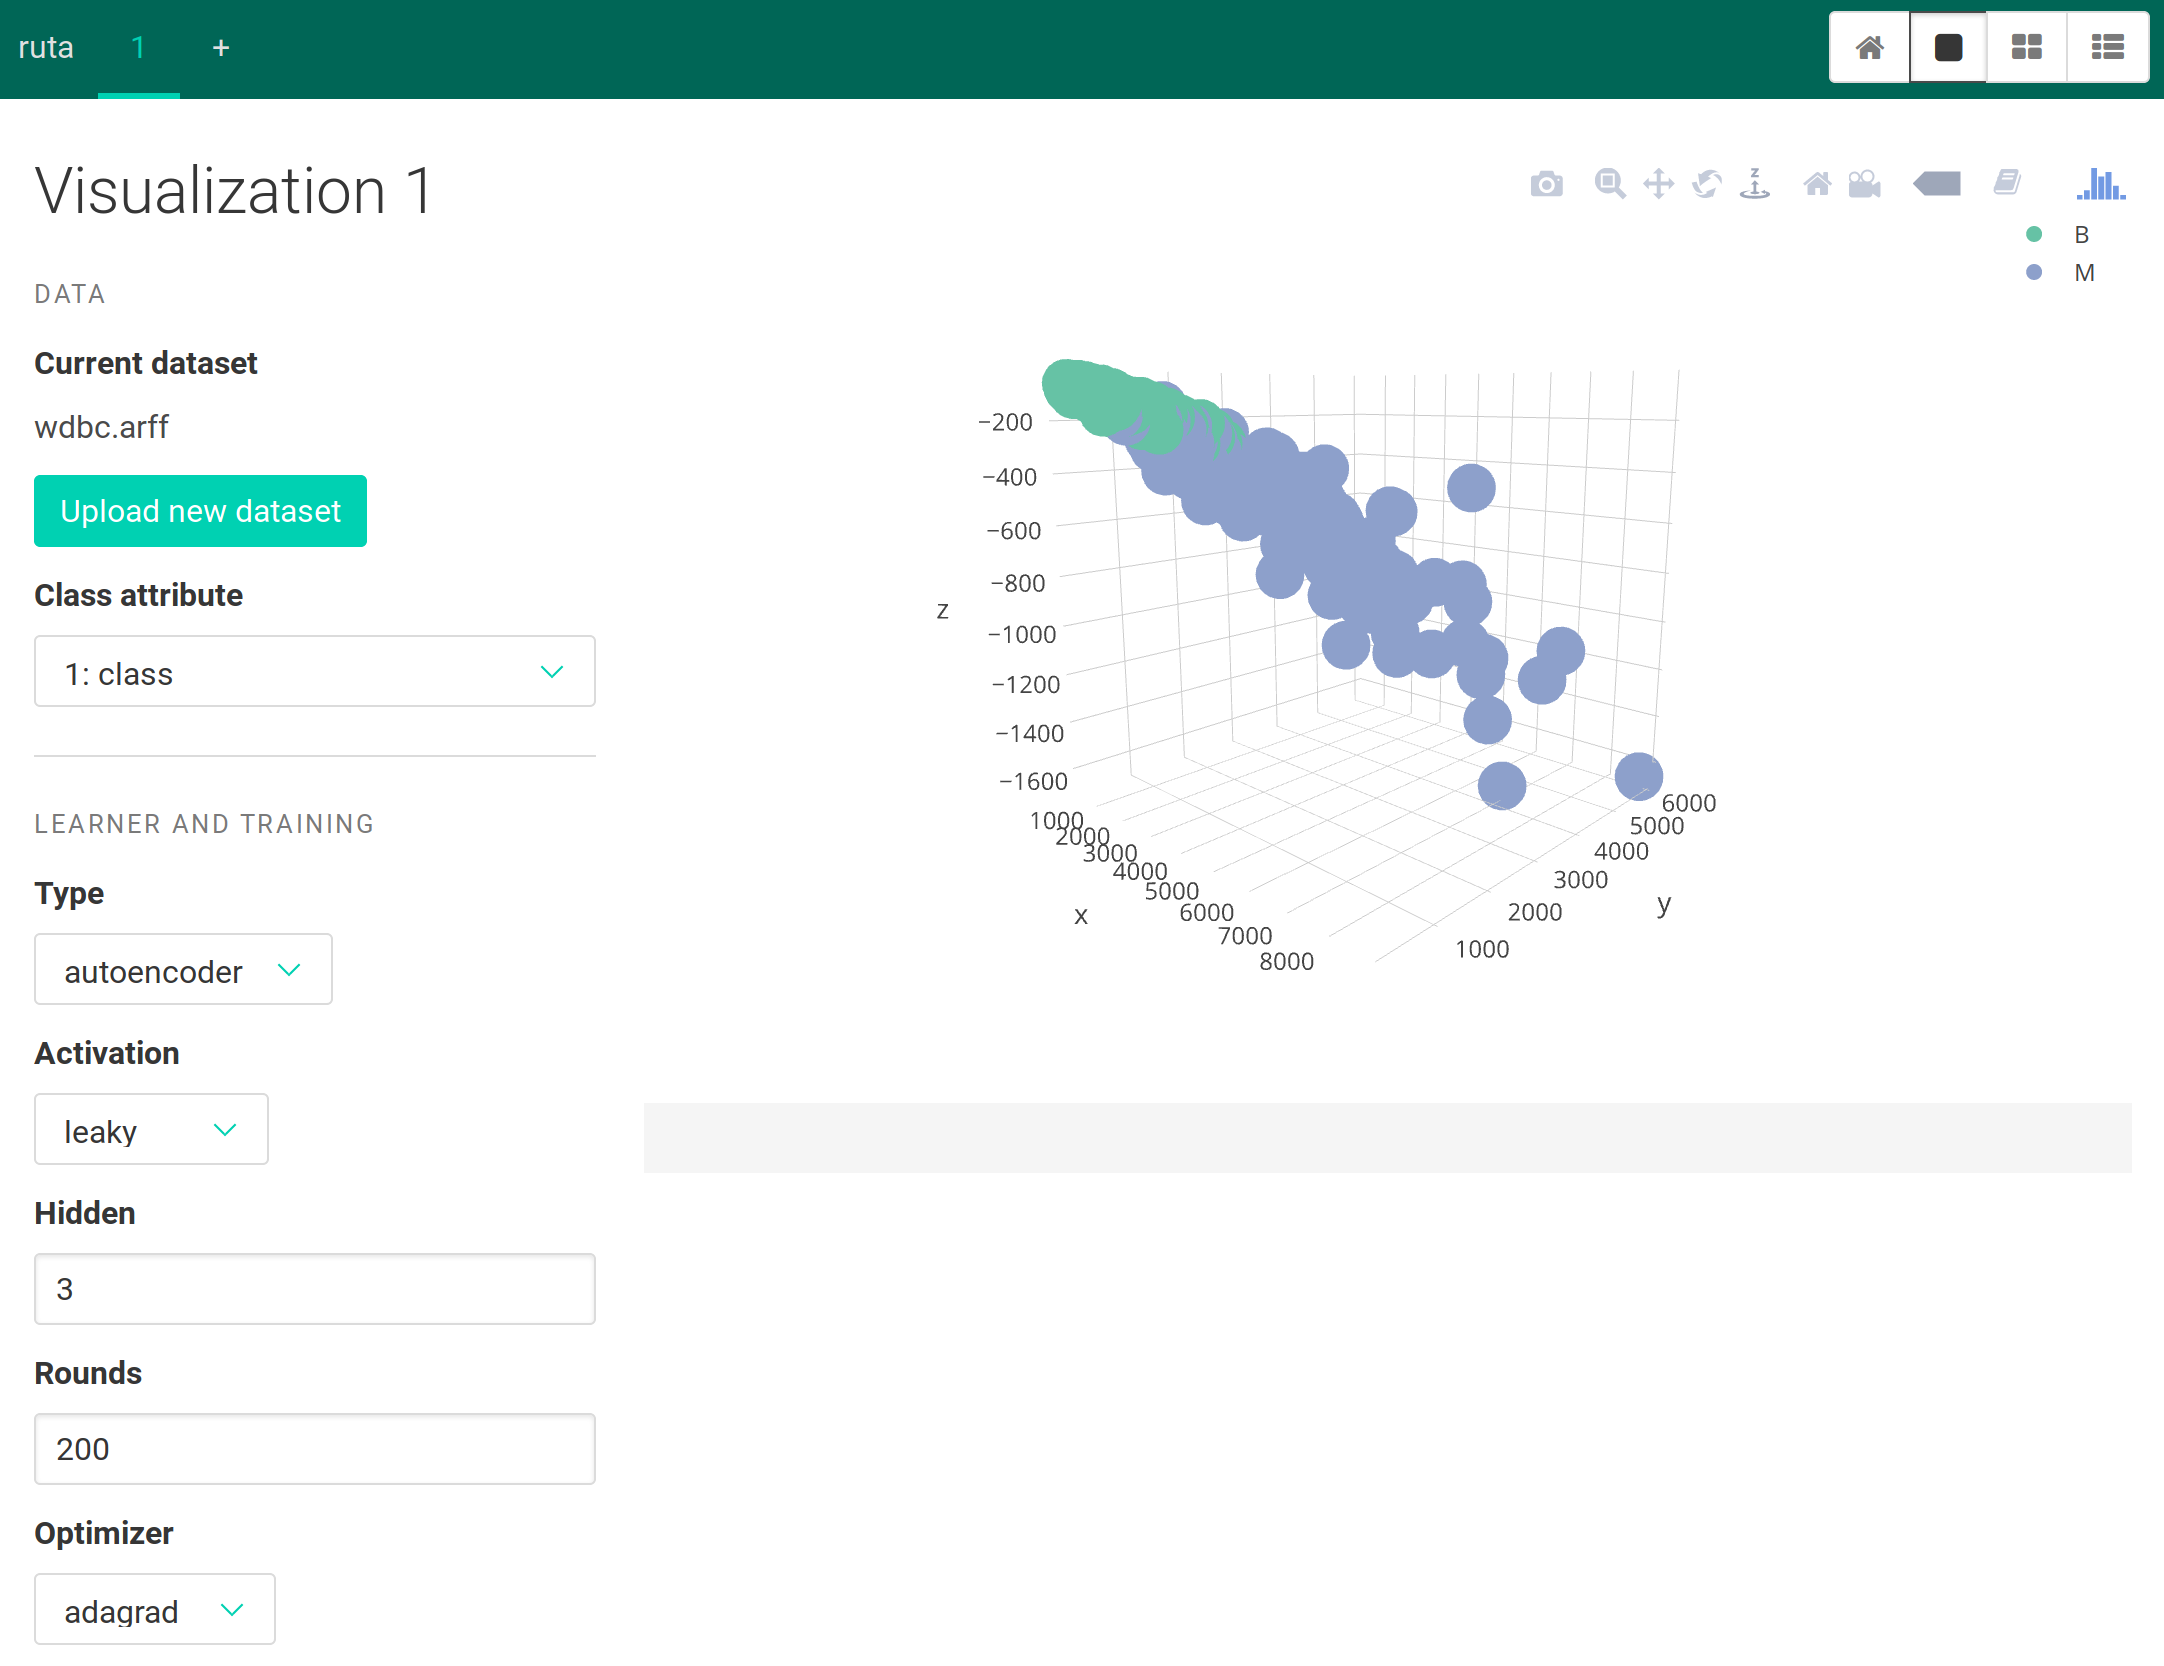
\includegraphics[width=\textwidth]{images/rutavis_plot2}}
  \caption[Interfaz gráfica de Rutavis]{Interfaz gráfica de usuario de Rutavis. Arriba, la barra de pestañas y modos de visualización. A la izquierda, ajuste de parámetros. En el centro, visualización de las gráficas generadas}
  \label{fig:rutavis1}
\end{figure}

Añadimos un segundo entorno de visualización mediante el botón \emph{+} de la barra superior de pestañas. Entrenamos un modelo similar, en este caso con unidades con función de activación tangente hiperbólica y distintos parámetros de épocas y tasa de aprendizaje. Seleccionamos la vista de mosaico para comparar ambos resultados, como se muestra en la \autoref{fig:rutavis3}. La vista estilo \emph{notebook} es similar a esta, pero apilando verticalmente todas las visualizaciones añadidas.

\begin{figure}[hbtp]
  \centering
  \fbox{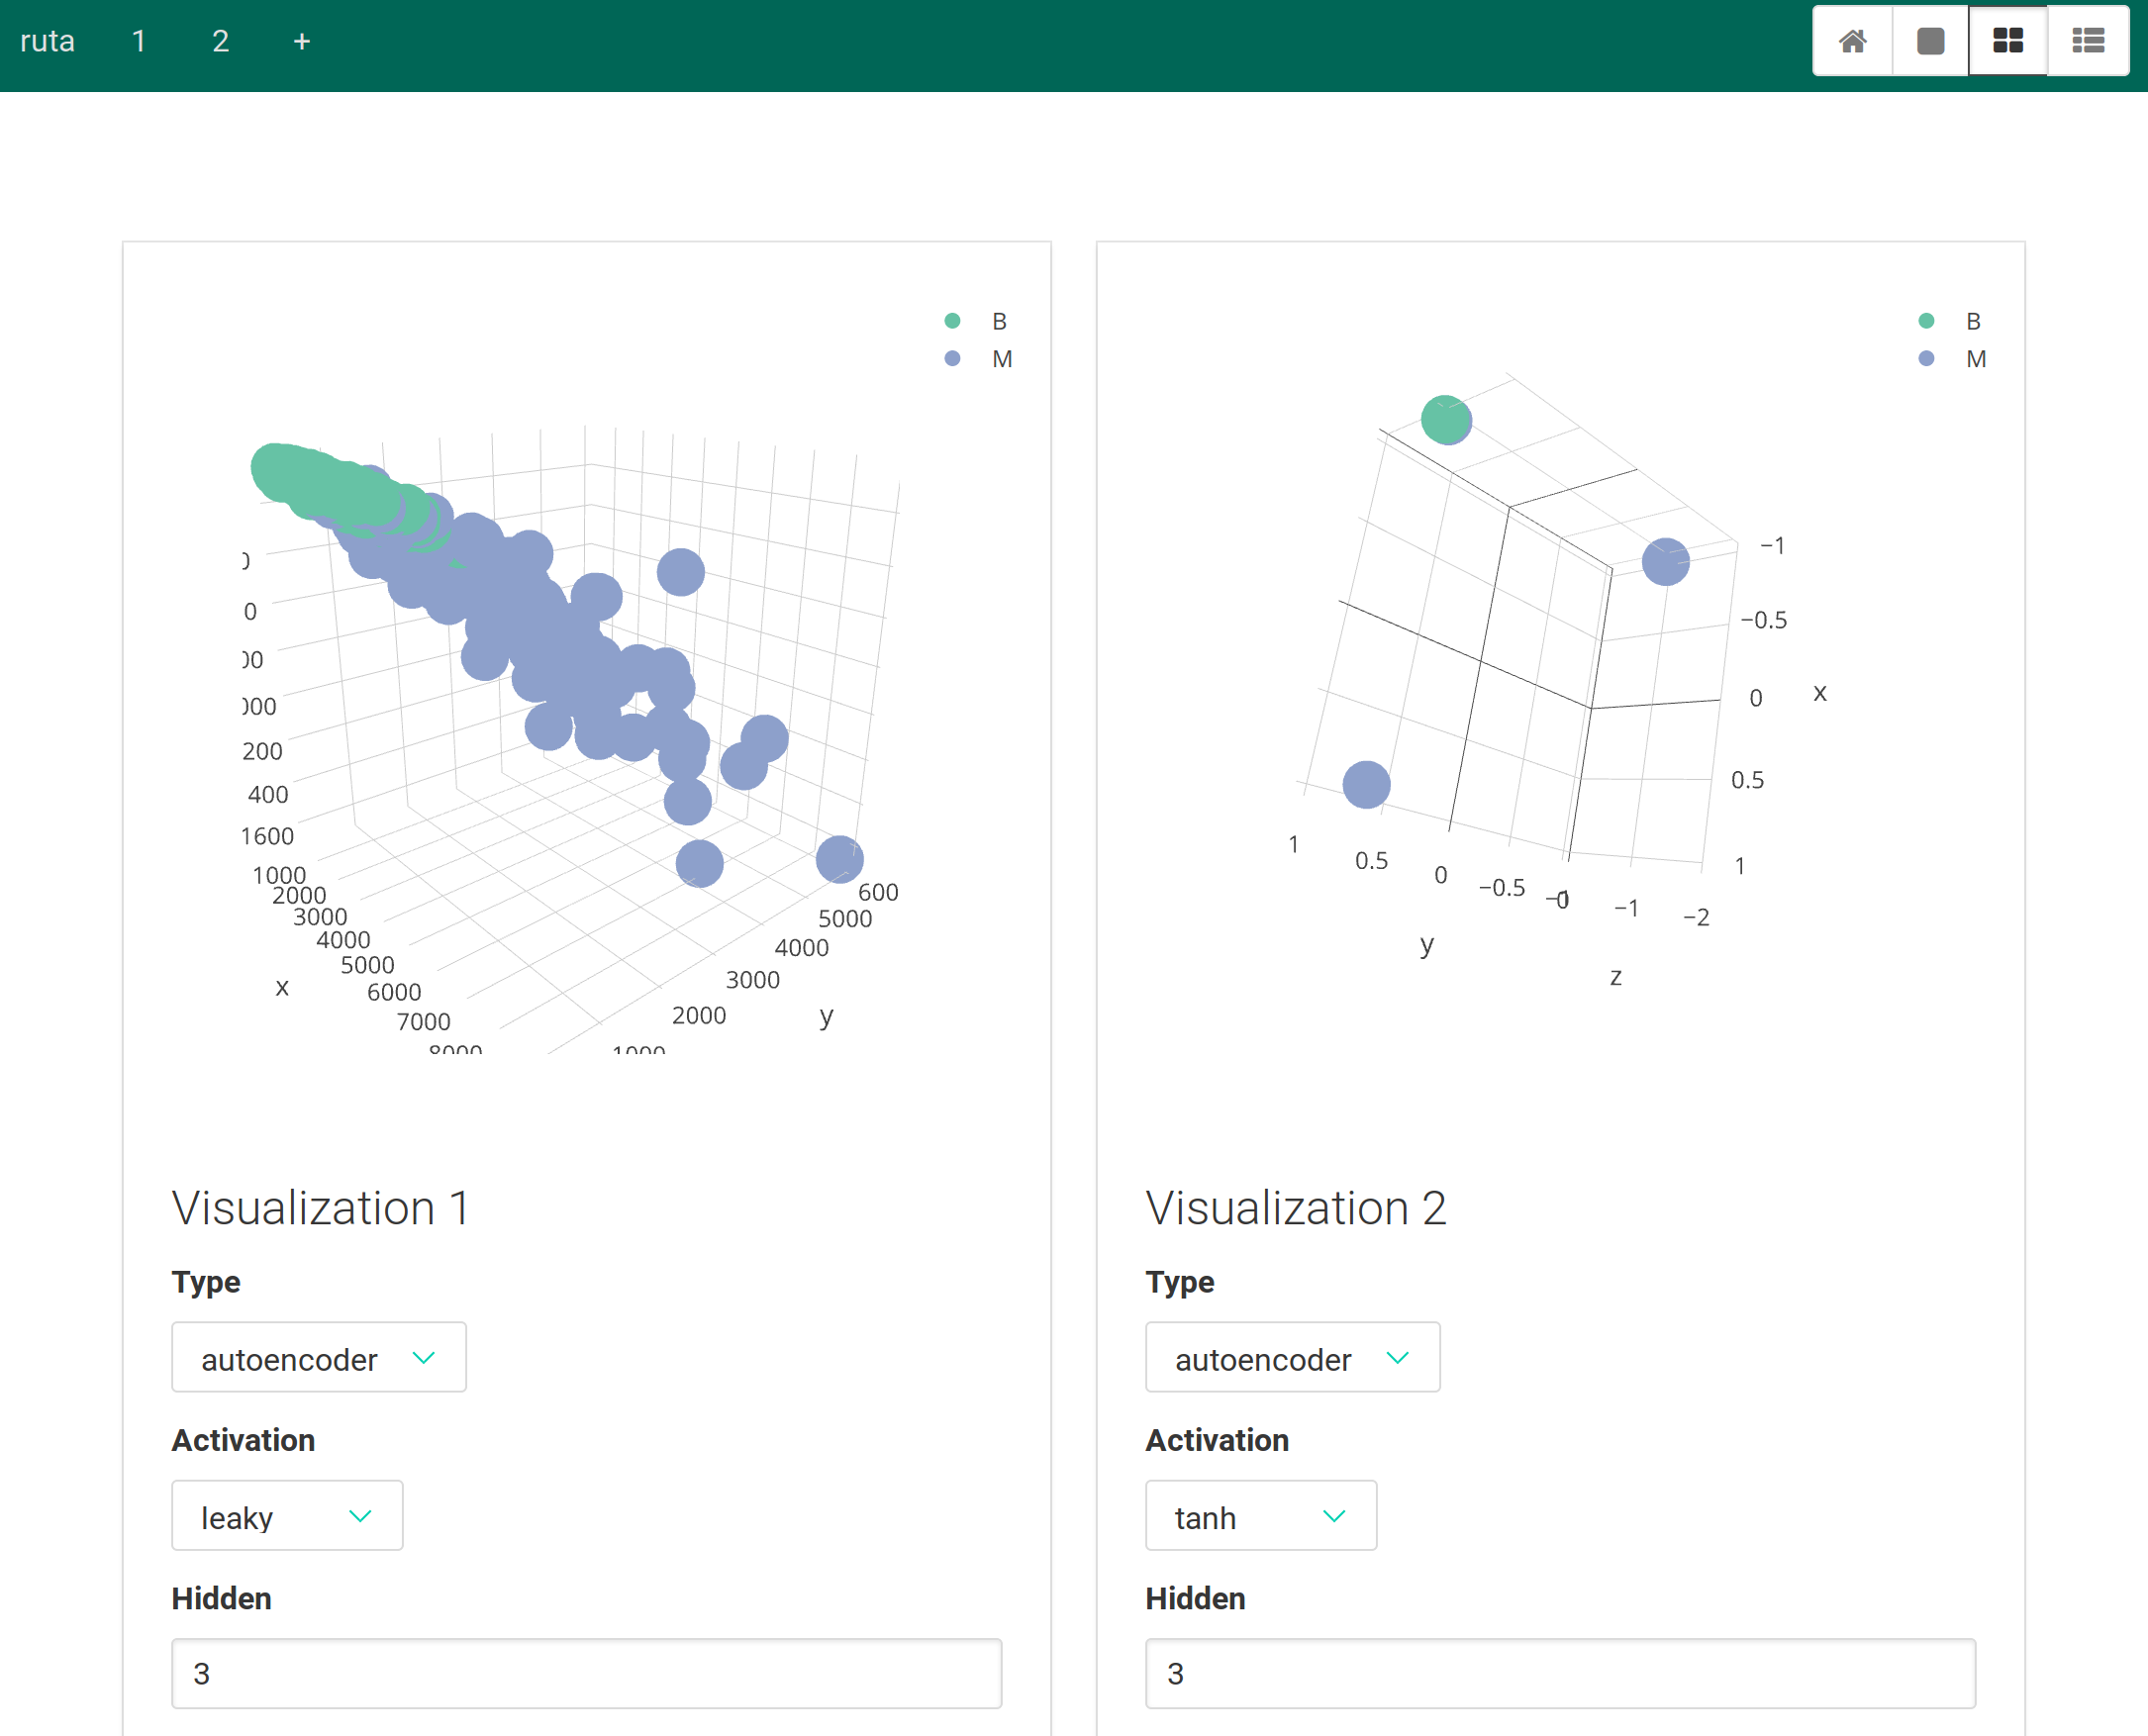
\includegraphics[width=\textwidth]{images/rutavis_compare}}
  \caption[Modo mosaico de Rutavis]{Comparación de dos visualizaciones en el modo mosaico de Rutavis}
  \label{fig:rutavis3}
\end{figure}